\chapter{METHODOLOGY}

\section{Research Design}

\begin{figure}[H]
	\raggedright
	\textbf{Figure 1} \\ % Figure number left-aligned
	\textit{Modified Waterfall Model of SDLC} % Title left-aligned

	\vspace{0.5em}
	\centering
	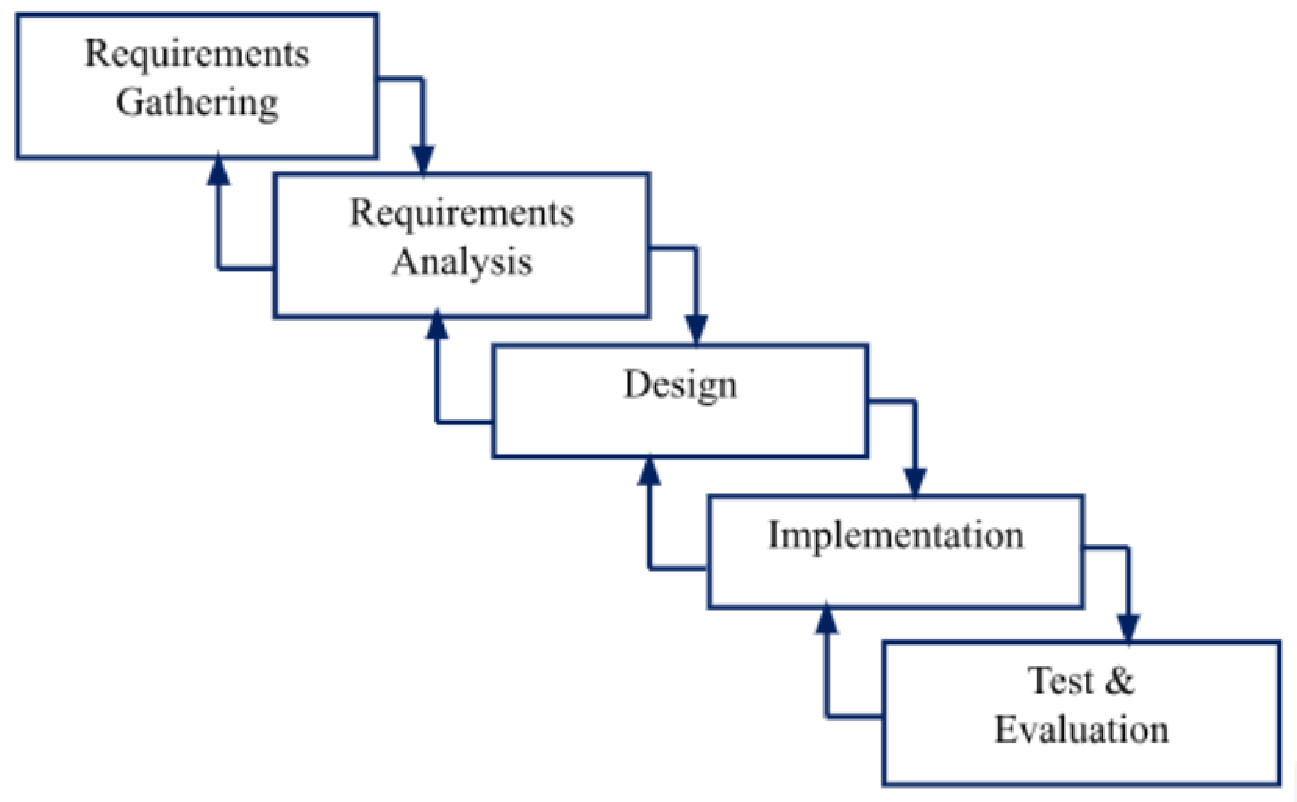
\includegraphics[width=0.9\textwidth]{figures/waterfall.pdf} % image

	\vspace{0.5em}
	\raggedright

	\label{fig:waterfall}
\end{figure}

The methodology has been adopted from the Modified Waterfall Model of the Systems Development Life Cycle (SDLC). The methodology is selected due to its structured yet flexible nature, allowing for sequential phases with opportunities for feedback and refinement. This is particularly important in agricultural technology development, where both technical precision and field validation are critical. For this study, it enables the researchers to systematically design, implement, and evaluate the integration of UAV-collected imagery with YOLO for early disease detection in cacao pods, ensuring that each phase is thoroughly reviewed before progressing to the next, while still accommodating necessary adjustments. Figure 2 shows the stages necessary for development.

\section{Requirements Gathering}
\subsection{Data Gathering}

To ensure a well-rounded and effective system design, data for this study will be collected from various relevant sources:
\subsection{Sources of Data}
\textbf{Cacao Farmers and Field Personnel}. Surveys and interviews will be conducted with cacao growers and farm workers to gather insights on existing practices for disease detection, common issues encountered in the field, and expectations for a UAV-based detection system.

\textbf{Agricultural Specialists}. Input from agricultural professionals will be obtained to identify key disease symptoms, validate detection criteria, and provide guidance on effective monitoring strategies for cacao pod health.

\textbf{Existing Literature and Research Studies}. A comprehensive review of academic and technical literature, such as studies by Baculio \& Barbosa (2022), Vera et al. (2024), and Solpot (2020), will support the design of the detection system by offering benchmarks on accuracy, image processing, and the use of machine learning in agriculture.

\textbf{Technology Experts}. Consultations with UAV technicians, AI developers, and computer vision experts will be sought to ensure the system’s technological components such as image acquisition and model training are both feasible and optimized for agricultural environments.

\subsection{Data Gathering Procedure}

\textbf{Questionnaire}. A structured questionnaire will be distributed to cacao farmers and field personnel to gather information about their current practices in detecting cacao pod diseases, the challenges they face in early identification, and their perspectives on using UAV-based solutions. Before distribution, the questionnaire will be reviewed and approved by the research adviser, agricultural specialists, and academic authorities to ensure that it is technically sound, ethically appropriate, and aligned with the objectives of the study.

\textbf{Interview}. Interviews will be conducted with cacao farmers, agricultural experts, UAV technicians, and AI developers. These interviews aim to collect in-depth insights on disease symptoms, detection indicators, drone imaging strategies, and technical requirements.

\textbf{Existing Literature}. A review of relevant literature will be conducted to understand
the current state of disease detection systems in agriculture, particularly focusing on cacao
pod diseases. This will include studies on the use of UAVs, AI-driven disease detection
`odels (such as YOLO), and the challenges associated with deploying such technologies
in real-world farming environments. and provide a foundation for comparing the proposed
system with existing solutions.

\subsection{User Definition}
Following the requirements gathering process, the primary user of the system has been identified.

\textit{Farmers} - The primary user of the system, responsible for utilizing UAVs to detect early signs of cacao pod diseases and making informed decisions for crop management.

\begin{longtable}{p{4cm} p{8cm}}
	\caption{System Requirements} \label{tab:sysreq}                                                                                                                                      \\
	\toprule
	\textbf{Category}        & \textbf{System Requirements}                                                                                                                               \\
	\midrule
	\endfirsthead
	\toprule
	\textbf{Category}        & \textbf{System Requirements}                                                                                                                               \\
	\midrule
	\endhead
	\bottomrule
	\endfoot
	Input Requirements       & - The system shall collect images of cacao pods captured by UAVs for disease detection.                                                                    \\
	                         & - The system shall allow users to initiate UAV image capture and review sessions through a simple interface.                                               \\
	                         & - The system shall utilize annotated image datasets for training the AI model, specifically focusing on black pod disease.                                 \\
	                         & - The system shall use GPS metadata from UAVs as input to geo-tag disease detection results.                                                               \\
	\midrule
	Process Requirements     & - The system shall process captured images using the YOLO model to identify and classify diseased cacao pods.                                              \\
	                         & - The system shall preprocess input images for consistency.                                                                                                \\
	                         & - The system shall utilize a labeled image dataset of cacao pods.                                                                                          \\
	                         & - The system shall include a manual annotation process where images are labeled with infection presence and location.                                      \\
	\midrule
	Output Requirements      & - The system shall display detection results, highlighting infected areas on cacao pods in real-time or after processing.                                  \\
	                         & - The system shall classify each detected pod as either healthy or infected.                                                                               \\
	                         & - The system shall provide GPS coordinates alongside detection results for mapping infected areas.                                                         \\
	                         & - The system shall generate summary reports including: total number of pods detected, number and percentage of infected pods, detection time and location. \\
	\midrule
	Control Requirements     & - The system shall implement secure access with user authentication to ensure that only authorized users (farmers) can access the system.                  \\
	                         & - The system shall maintain logs of image captures, analysis sessions, and user feedback for audit and traceability.                                       \\
	                         & - The system shall validate all image inputs and user entries to ensure accurate and usable data is processed.                                             \\
	\midrule
	Performance Requirements & - The system shall be capable of processing high resolution images in real-time or near real-time with minimal latency.                                    \\
	                         & - The system shall efficiently manage and store large datasets of images and detection results, supporting scalable usage over time.                       \\
	                         & - The system shall maintain uptime and availability to ensure uninterrupted use during farming operations.                                                 \\
\end{longtable}

\section{Requirements Analysis}
\subsection{Data Finding Analysis}

\textbf{Qualitative Analysis}. Thematic analysis will be applied to interviews and open-ended survey responses. This approach will help identify recurring themes such as difficulties in manual disease detection, trust in machine learning techniques, and challenges related to the adoption of UAVs. Insights from this analysis will inform user-centered system design and guide improvements in usability and functionality.

\textbf{Quantitative Analysis}. Descriptive statistical analysis will be used for the structured survey data. This includes calculating frequencies, percentages, and average values to measure levels of technological readiness, prevalence of black pod disease, and the willingness of users to adopt UAV-based solutions for monitoring. These metrics will provide measurable indicators to support system feature prioritization.


\textbf{Feasibility Analysis}. Hardware specifications and machine learning model performance will be assessed through expert consultations and a review of relevant literature. This includes evaluating the accuracy of YOLO for disease detection and the practicality of drone operation in cacao farm environments using a performance matrix.

\textbf{Spatial Analysis}. Given that the UAV system captures geo-tagged images, spatial analysis will be conducted to examine the geographical distribution of detected disease cases. This analysis will help visualize infection hotspots across the farm and support precision intervention strategies.

\section{Design and Implementation}

\subsection{Context Level Diagram}

\begin{figure}[H]
	\raggedright
	\textbf{Figure 2} \\ % Figure number left-aligned
	\textit{Context Level Diagram of the Study} % Title left-aligned

	\vspace{0.5em}
	\centering
	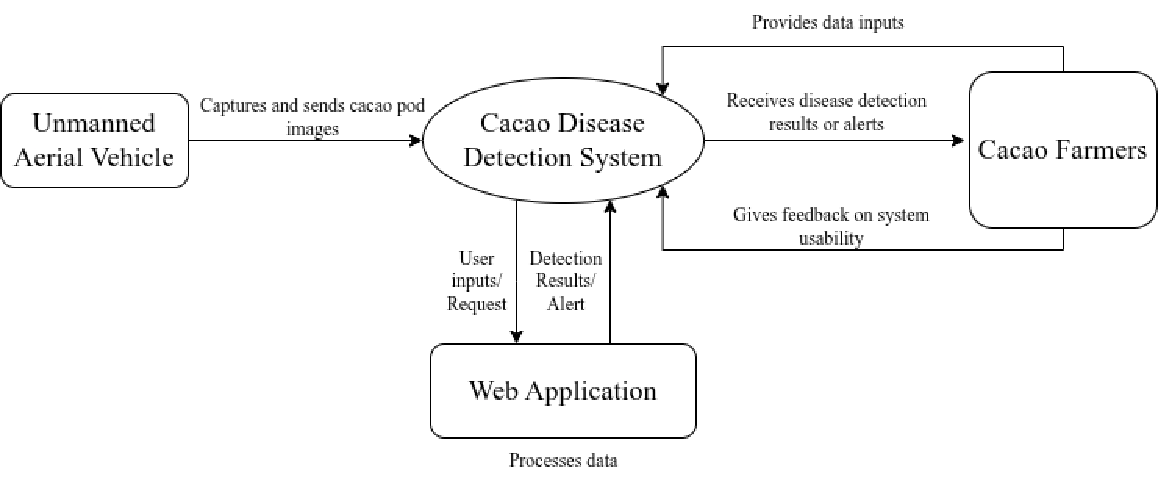
\includegraphics[width=0.9\textwidth]{figures/Context-Level.pdf} % image

	\vspace{0.5em}
	\raggedright

	\label{fig:context-level}
\end{figure}

Figure 2 illustrates the context-level diagram of the cacao disease detection system. This diagram provides a high-level overview of the interactions. As a context-level diagram, it abstracts away internal processing to focus solely on how external entities interact with the system as a whole. The system integrates an Unmanned Aerial Vehicle (UAV), which is responsible for capturing and transmitting aerial imagery of cacao pods. These images serve as critical input for the system’s disease detection processes. The Web Application functions as the user interface, facilitating communication between the system and its users. Through this platform, cacao farmers can input relevant field data and observations, while also receiving timely detection results. Cacao farmers contribute to the system by using the web app, submitting field data, and providing feedback for continuous improvement.

\subsection{System Architecture}

\begin{figure}[H]
	\raggedright
	\textbf{Figure 3} \\ % Figure number left-aligned
	\textit{System Architecture of the Study} % Title left-aligned

	\vspace{0.5em}
	\centering
	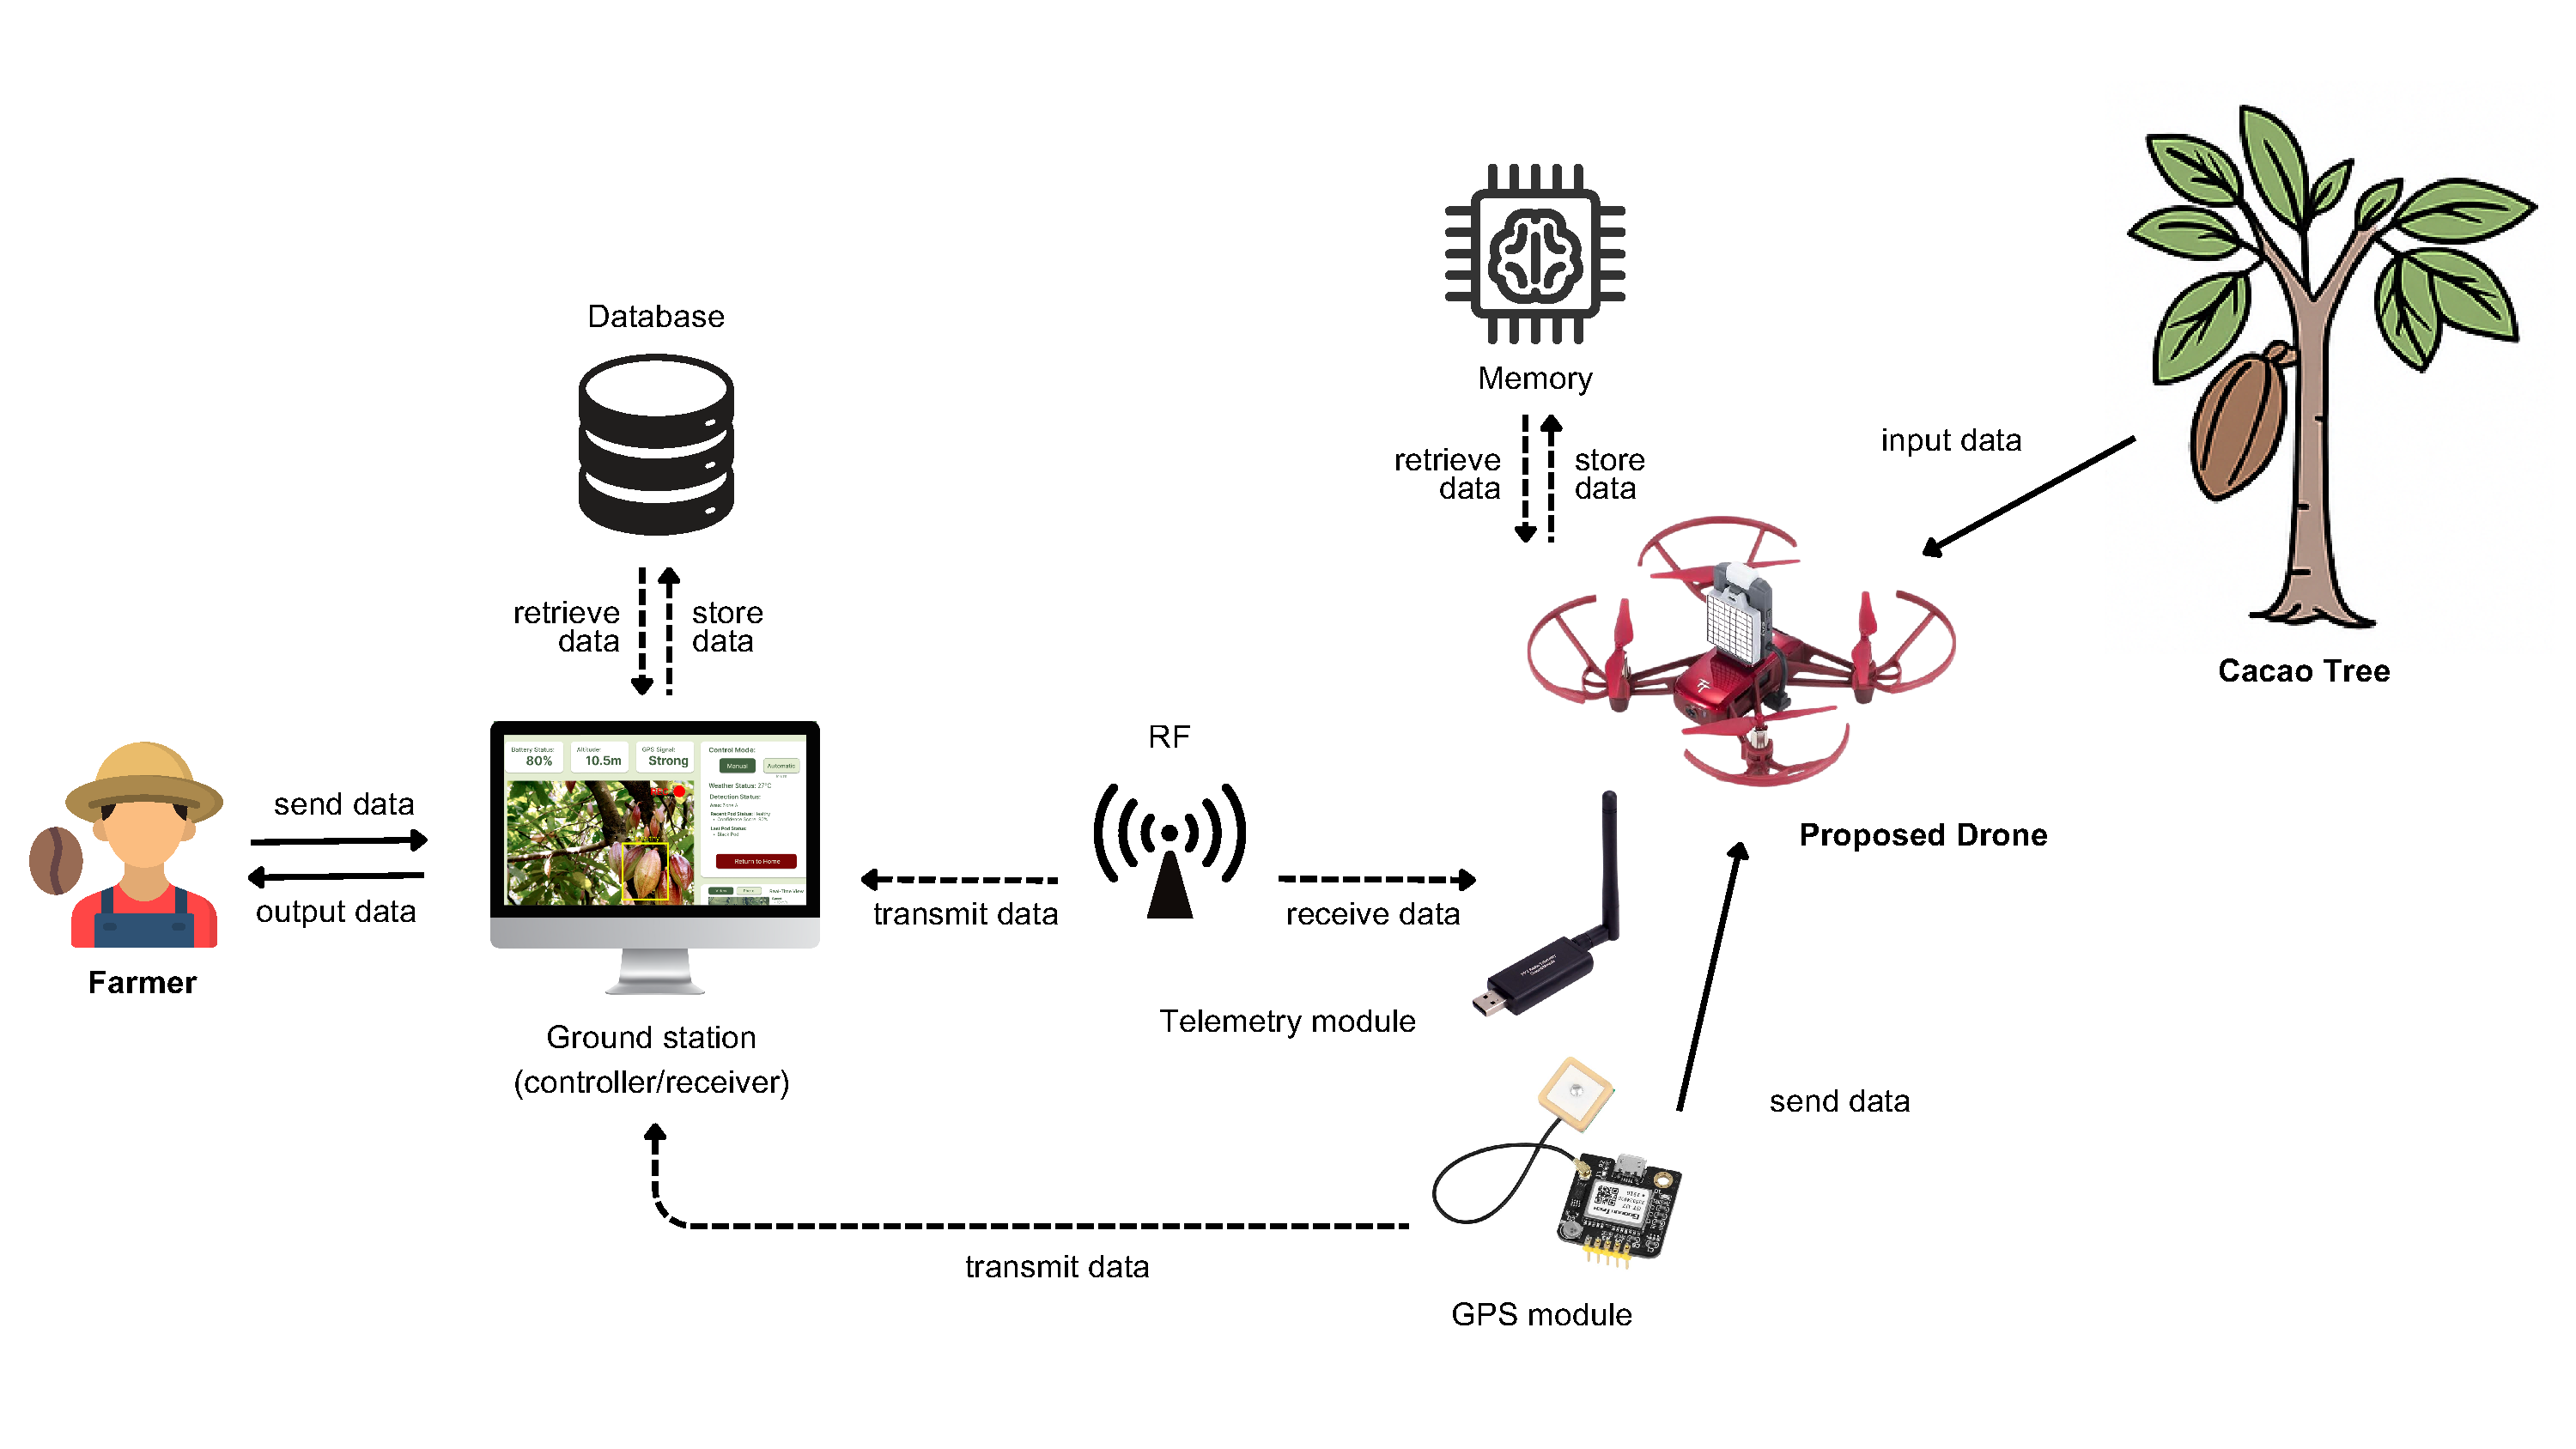
\includegraphics[width=0.9\textwidth]{figures/SysArch.pdf} % image

	\vspace{0.5em}
	\raggedright

	\label{fig:SysArch}
\end{figure}

Figure 3 illustrates the system architecture of the study. The process begins with the cacao trees, which are the central focus of the system. To monitor them, a proposed drone is deployed over the farm. This DJI RoboMaster TT is equipped with cameras and sensors that collect input data—primarily images and environmental readings—from the trees as it flies at the same level as them. The data captured by the drone is transmitted to an open-source controller with a camera module, which acts as the drone’s mini computer. This device processes the incoming images and sensor data. Additionally, a GPS module connected to the system sends precise geolocation data to the processor, tagging the collected images with accurate coordinates. Once the data is processed, it is temporarily stored in a memory unit. From there, the data is transmitted using a telemetry module, which serves as a bridge between the drone and the ground systems. The telemetry module sends the data wirelessly via RF to the web-based system, which acts as both a controller and a receiver. It receives the telemetry data and displays it in a user-friendly format, allowing the farmer to monitor the status of the cacao trees. The farmer can also send commands or control inputs back to the system using the system. All this information can be stored and retrieved from a database for later analysis or reference. The farmer is empowered with clear insights about the farm’s condition without needing to be physically present at each tree.

\subsection{Graphical User Interface (GUI)}
Figure 4 presents the proposed Dashboard interface for cacao disease detection. The dashboard is designed to summarize critical field data in a user-friendly format, supporting timely decision-making. The top section displays pod health statistics, including the number of black pods, healthy pods, and the total detected. At the center, a satellite image visualizes drone-analyzed areas with markers indicating infected zones. A pie chart provides a comparative view of healthy versus diseased pods across zones, while a detection history log on the right records recent findings with timestamps to enhance traceability and monitoring.

\subsection{Hardware and Software Requirements}

\begin{table}[H]
	\centering
	\caption{Hardware Requirements}
	\label{tab:hardreq}
	\begin{tabular}{ll}
		\toprule
		Drone      & DJI Robomaster TT (Tello Talent) \\
		\midrule
		GPS Module & NEO-M8N                          \\
		\bottomrule
	\end{tabular}
\end{table}

The hardware setup, summarized in Table 2, is composed of essential components that enable efficient data acquisition and geospatial referencing. The DJI RoboMaster TT (Tello Talent) drone is employed to capture aerial images of cacao pods, providing a stable and programmable platform for image collection. To ensure accurate geolocation tagging of each captured image, a NEO-M8N GPS module is integrated into the system. This GPS module delivers high-precision positional data, which enhances the reliability of spatial mapping and supports the alignment of imagery with corresponding field coordinates.

\begin{table}[H]
	\centering
	\caption{Software Requirements}
	\label{tab:softreq}
	\begin{tabular}{ll}
		\toprule
		Front-end               & Vue.js     \\
		\midrule
		Back-end                & Django     \\
		\midrule
		Database                & PostgreSQL \\
		\midrule
		API                     & QGIS       \\
		\midrule
		Web Server              & Nginx      \\
		\midrule
		Deep Learning Framework & YOLO       \\
		\bottomrule
	\end{tabular}
\end{table}

The software requirements, summarized in Table 3, specify the technologies utilized for interface development, system management, data storage, and disease detection. The front-end interface is built with Vue.js to enable user interaction and data visualization, while the back-end is powered by the Django framework, which manages system logic, workflows, and API integration. PostgreSQL functions as the primary database, storing user information, detection outputs, and geospatial metadata. Geospatial analysis and visualization of infected areas are facilitated through QGIS integration. The application is deployed using the Nginx web server to ensure efficient and reliable performance. For image-based disease detection, YOLO is implemented to process aerial imagery and identify signs of infection in cacao pods.

\section{Prototype}
The prototype phase will follow a structured approach focused on dataset collection, geotagging and mapping, sequence diagram, and system prototype.

\subsection{Data Collection}
A custom dataset will be generated using images captured by a DJI RoboMaster TT’s built-in camera during scheduled flights over cacao plantations. Capturing images from multiple angles and altitudes further enhances the dataset’s comprehensiveness and reliability. To ensure the model performs well in diverse real-world conditions, the dataset will include a broad range of images representing both healthy and diseased cacao pods. Data will be gathered under varying lighting conditions, weather scenarios, and backgrounds to promote generalizability and robustness in the detection process. Special attention will be given to capturing stages of infection, and degrees of pod visibility. All images will be manually annotated to label regions of interest, which is essential for supervised training of the YOLO model. The quality and accuracy of these annotations directly impact the model’s ability to detect and classify diseases reliably. Image preprocessing techniques such as resizing, normalization, and data augmentation may also be applied to enhance the dataset and prevent overfitting. Once prepared, the dataset will be used to train the YOLO detection model, forming the core component of the disease recognition system.

\subsection{Geotagging and Mapping}
To support spatial accuracy and enhance the traceability of captured data, geotagging and mapping functionalities are incorporated into the system architecture. A GPS module (NEO-M8N) is integrated with DJI RoboMaster TT open-source controller, enabling the synchronous acquisition of geographic coordinates during drone operations. As images are captured by the drone’s onboard camera, corresponding latitude and longitude values are simultaneously recorded and transmitted to the database. This ensures that each image can be accurately associated with its physical location within the cacao plantation. For spatial data visualization, the system employs the QGIS API, an open-source geographic information system that facilitates the rendering of geospatial information. Through this integration, users are able to interact with an intuitive map interface displaying drone flight paths, image capture points, and disease detection zones.

\subsection{Command-based Mission Control with Robomaster TT SDK}
Software Development Kit will be utilized in this study to implement command-based mission planning with the DJI RoboMaster TT. Through the SDK, the drone can execute scripted flight commands such as takeoff, forward(x), back(x), cw(angle), and land, enabling it to follow predefined flight paths across cacao rows. During these missions, the drone will capture images of cacao pods at specific intervals, which are then paired with location data provided by the integrated NEO-M8N GPS module. Unlike real-time processing systems, this study adopts an offline detection approach, where the collected images and GPS coordinates are stored and later processed using the YOLO algorithm. The results of the detection are then mapped in QGIS to identify and visualize areas affected by Phytophthora palmivora. This method allows the researchers to demonstrate a functional mission planning workflow that synchronizes drone navigation, image acquisition, and geotagging, while accounting for the RoboMaster TT’s hardware limitations.

\subsection{Flowchart of Hardware and Software}

\begin{figure}[H]
	\raggedright
	\textbf{Figure 5} \\ % Figure number left-aligned
	\textit{Hardware Flowchart} % Title left-aligned

	\vspace{0.5em}
	\centering
	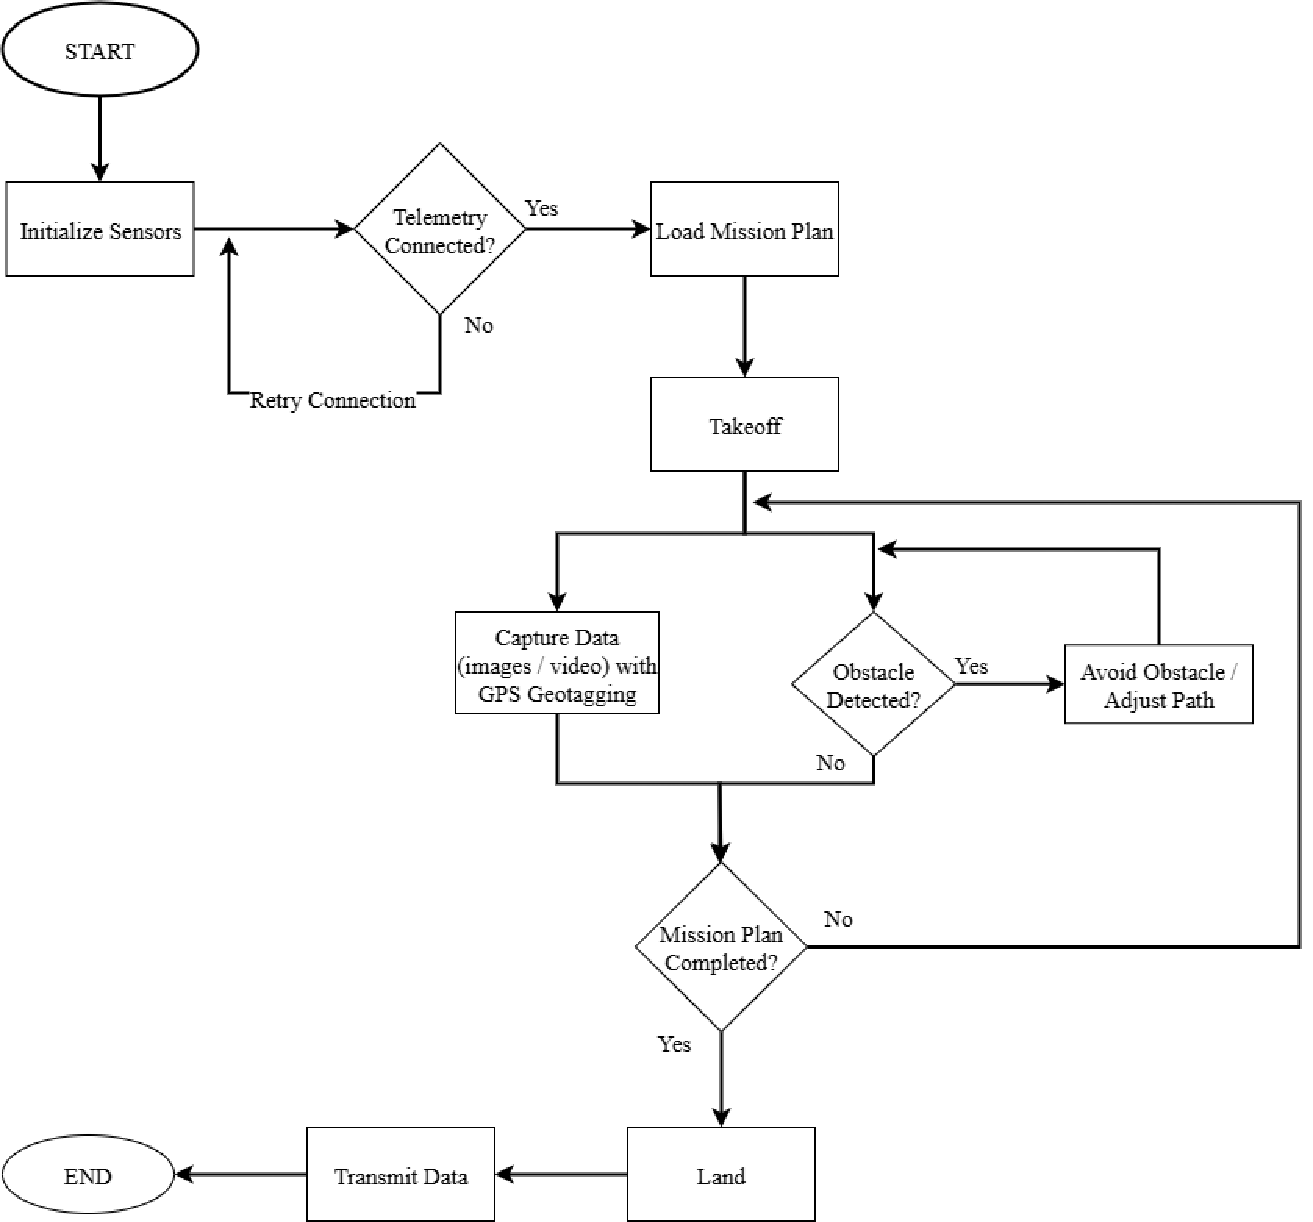
\includegraphics[width=0.9\textwidth]{figures/HardFlow.pdf} % image

	\vspace{0.5em}
	\raggedright

	\label{fig:HardFlow}
\end{figure}

Figure 5 illustrates the operational workflow of the UAV system; it begins with powering on the UAV, followed by the initialization of its key sensors, including the camera, GPS module, and obstacle detection system. Once the sensors are active, the system checks for telemetry connectivity with the ground station; if the connection fails, the drone retries until successful. After establishing a link, the mission plan is loaded from the ground station, and the UAV proceeds to takeoff. During flight, two processes run in parallel: the drone continuously captures images and videos with GPS geotags for later processing, while simultaneously monitoring its environment for obstacles and adjusting its path when necessary. The system then checks whether the mission plan has been completed. If it is complete, the UAV proceeds to land; if not, it continues executing the remaining tasks until completion. Only after landing are the stored image and location data transmitted to the ground station for processing. The operation then concludes with system power down.

\begin{figure}[H]
	\raggedright
	\textbf{Figure 6} \\ % Figure number left-aligned
	\textit{Software FlowChart} % Title left-aligned

	\vspace{0.5em}
	\centering
	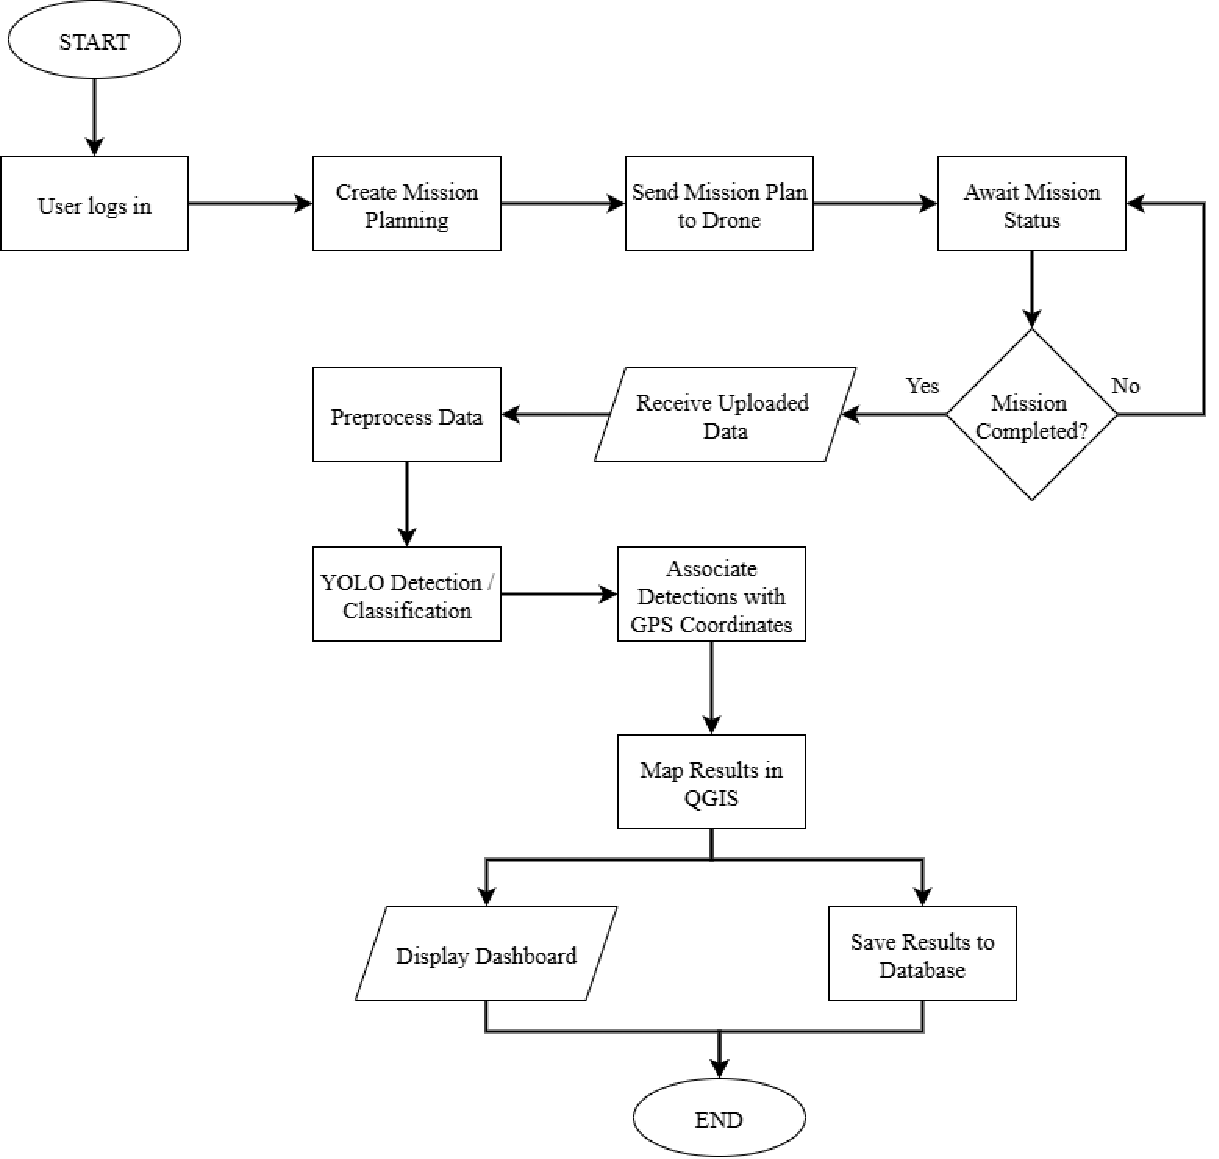
\includegraphics[width=0.9\textwidth]{figures/SoftFlow.pdf} % image

	\vspace{0.5em}
	\raggedright

	\label{fig:SoftFlow}
\end{figure}

Figure 6 shows the software workflow, starting with the user logging into the system and creating a mission plan that defines waypoints, altitude, and capture intervals. This plan is then sent to the UAV through SDK, after which the system awaits mission status updates. At this stage, a decision point determines whether the mission has been completed. If the mission is successful, the system retrieves the uploaded images with their GPS metadata; otherwise, it continues waiting until completion. Once the data is received, the images undergo preprocessing such as resizing, normalization, and augmentation before being passed through the YOLO algorithm for disease detection and classification. The detection results are then associated with GPS coordinates to ensure spatial accuracy and are mapped in QGIS to generate a clear visualization of affected areas. From this stage, two operations run in parallel: results are displayed on the dashboard for immediate user insight, while the same results are saved into the database for reporting and long-term storage. Finally, the processes converge, and the mission concludes to complete the workflow.

\section{Testing}
Testing was conducted to ensure that the system operates accurately, efficiently, and is suitable for real-world use in cacao farm management. The process involved functional testing, usability testing, and performance testing. Functional testing verified whether key features—such as UAV image capture, detection of Phytophthora palmivora-infected cacao pods using the YOLO, and geotagging of infected trees—performed as intended, with each function tested through defined inputs and expected outputs. Usability testing assessed how easily end users, particularly cacao farmers, could navigate and interact with the system by performing essential tasks such as logging in, accessing detection results, and interpreting geotagged maps. Feedback was collected using the System Usability Scale (SUS) to evaluate the overall user experience. Performance testing measured the system’s responsiveness and accuracy, focusing on the time taken from image capture to the display of results, as well as the efficiency in processing high-resolution images and managing data. Together, these tests validated the system’s reliability, user-friendliness, and effectiveness in supporting early disease detection and timely intervention.

\subsection{Functional Testing}
Functional testing will be carried out to ensure that every part of the system works as intended. This testing will begin once the prototype is complete. It will focus on verifying key features, such as capturing images through the drone, detecting healthy and infected cacao pods using the YOLO, tagging infected trees’ locations with GPS, and displaying results clearly on the dashboard. Each function will be tested by giving specific inputs and checking if the outputs match what is expected. For example, the drone should respond correctly to manual and automatic commands, and the system should accurately identify pods and show their locations on the map. This testing helps find and fix any errors or missing functions, making sure the system is reliable and ready for real-world use.

\subsection{Usability Testing}
Usability testing will be conducted to make sure the system is easy and practical for cacao farmers to use. After the prototype is ready, farmers will be invited to try important features such as logging in, flying the drone, viewing pod detection results, and checking the map showing infected trees. After using the system, they will fill out a short survey called the System Usability Scale (SUS), which measures how user-friendly the system feels. The survey uses a rating scale from 1 to 5 and asks about how easy the system is to learn, how confident they feel using it, and whether the features work well together. Scores are converted to a total out of 100, with scores above 68 generally meaning the system is easy to use. This process will help the team understand what works well and what needs improvement before the system is fully deployed.

\subsection{Performance Testing}

Performance testing is conducted to evaluate the system’s responsiveness, accuracy, and overall reliability based on its core functionalities. This includes measuring the accuracy of detecting Phytophthora palmivora-infected cacao pods using the YOLO, assessing the precision of geolocation through GPS module and QGIS, and recording the system’s response time from image capture to the display of results on the dashboard. The test is carried out under standard operating conditions to determine whether the system can process high-resolution images efficiently and deliver real-time outputs. The results of this evaluation are essential in verifying that the system meets its intended performance criteria and is capable of supporting timely and informed decision-making in cacao disease management.

